
\chapter{\gramSchmidtTitle}\label{gramschmidt}


Given a vector $v$ and some other vector $u$ not in  $ {\rm span}\, \{v\} $, we can construct a new vector: 
\[
v^\perp:=v-\frac{u\cdot v}{u\cdot u}u.
\]
\begin{center}
\input{vperp.pdftex_t}
\end{center}
This new vector $v^\perp$ is orthogonal to $u$ because 
\[
u\dotprod v^\perp = u\dotprod v - \frac{u\cdot v}{u\cdot u}u\dotprod u = 0.
\]
Hence, $\{u, v^\perp\}$ is an orthogonal basis for $\spa \{u,v\}$.  When $v$ is not parallel to $u$, $v^\perp \neq 0$, and normalizing these vectors we obtain $\left\{\frac{u}{|u|}, \frac{v^\perp}{|v^\perp|} \right\}$, an orthonormal basis for the vector space ${\rm span}\, \{u,v\}$.

Sometimes we write $v = v^\perp + v^\parallel$ where:
\begin{eqnarray*}
v^\perp &=& v-\frac{u\cdot v}{u\cdot u}u \\
v^\parallel &=& \phantom{v-}\frac{u\cdot v}{u\cdot u}u.
\end{eqnarray*}
This is called an \emph{orthogonal decomposition}\index{Orthogonal decomposition} because we have decomposed $v$ into a sum of orthogonal vectors.  This decomposition depends on $u$; if we change the direction of $u$ we change $v^\perp$ and $v^\parallel$.

If $u$, $v$ are linearly independent vectors in $\Re^3$, then the set $\{u, v^\perp, u\times v^\perp \}$ would be an orthogonal basis for $\Re^3$.  This set could then be normalized by dividing each vector by its length to obtain an orthonormal basis.

However, it often occurs that we are interested in vector spaces with dimension greater than $3$, and must resort to craftier means than cross products to obtain an orthogonal basis.
\footnote{Actually, given a set $T$ of $(n-1)$ independent vectors in $n$-space, one can define an analogue of the cross product that will produce a vector orthogonal to the span of $T$, using a method exactly analogous to the usual computation for calculating the cross product of two vectors in $\Re^3$.  This only gets us the \emph{last} orthogonal vector, though; the process in this Section gives a way to get a full orthogonal basis.}
%yeah, and who is going to teach them about the Hodge star in office hours? I say nix this footnote -cherney

Given a third vector $w$, we should first check that $w$ does not lie in the span of $u$ and $v$, \textit{i.e.} check that $u,v$ and $w$ are linearly independent.   We then can define:
\[
w^\perp = w - \frac{u\dotprod w}{u\dotprod u}\,u - \frac{v^\perp\dotprod w}{v^\perp\dotprod v^\perp}\,v^\perp.
\]

We can check that \(u \dotprod w^\perp\) and \(v^\perp \dotprod w^\perp\) are both zero:
\begin{align*}
u \dotprod w^\perp&=u \dotprod \left(w - \frac{u\dotprod w}{u\dotprod u}\,u - \frac{v^\perp\dotprod w}{v^\perp\dotprod v^\perp}\,v^\perp \right)\\&= u\dotprod w - \frac{u \dotprod w}{u \dotprod u}u \dotprod u - \frac{v^\perp \dotprod w}{v^\perp \dotprod v^\perp} u \dotprod v^\perp \\
&=u\dotprod w-u\dotprod w-\frac{v^\perp \dotprod w}{v^\perp \dotprod v^\perp} u \dotprod v^\perp\ =\ 0
\end{align*}
since \(u\) is orthogonal to \(v^\perp\), and
\begin{align*}
v^\perp \dotprod w^\perp&=v^\perp \dotprod \left(w - \frac{u\dotprod w}{u\dotprod u}\,u - \frac{v^\perp\dotprod w}{v^\perp\dotprod v^\perp}\,v^\perp \right)\\ &=v^\perp\dotprod w - \frac{u \dotprod w}{u \dotprod u}v^\perp \dotprod u - \frac{v^\perp \dotprod w}{v^\perp \dotprod v^\perp} v^\perp \dotprod v^\perp \\
&=v^\perp\dotprod w-\frac{u \dotprod w}{u \dotprod u}v^\perp \dotprod u - v^\perp \dotprod w\ =\ 0
\end{align*}
because \(u\) is orthogonal to \(v^\perp\). Since $w^\perp$ is orthogonal to both $u$ and $v^\perp$, we have that $\{u,v^\perp,w^\perp \}$ is an orthogonal basis for $\spa \{u,v,w\}$.

\section{The Gram-Schmidt Procedure}
In fact, given a set $\{v_1, v_2, \ldots \}$ of linearly independent vectors, we can define an orthogonal basis for $\spa \{v_1,v_2, \ldots \}$ consisting of the following vectors:
\begin{eqnarray*}
v_1^\perp&:=&v_1 \\
v_2^\perp &:=& v_2 - \frac{v_1^\perp\cdot v_2}{v_1^\perp\cdot v_1^\perp}\,v_1^\perp \\
v_3^\perp &:=& v_3 - \frac{v_1^\perp\cdot v_3}{v_1^\perp\cdot v_1^\perp}\,v_1^\perp - \frac{v_2^\perp\cdot v_3}{v_2^\perp\cdot v_2^\perp}\,v_2^\perp\\
&\vdots& \\
v_i^\perp%&=&   v_i - \sum_{j<i} \frac{v_j^\perp\cdot v_i}{v_j^\perp\cdot v_j^\perp}\,v_j^\perp \\
 &:=& v_i - \frac{v_1^\perp\cdot v_i}{v_1^\perp\cdot v_1^\perp}\,v_1^\perp -  
 - \frac{v_2^\perp\cdot v_3}{v_2^\perp\cdot v_2^\perp}\,v_2^\perp -\cdots
 - \frac{v_{i-1}^\perp\cdot v_i}{v_{i-1}^\perp\cdot v_{i-1}^\perp}\,v_{i-1}^\perp\\
&\vdots& \\
\end{eqnarray*}
Notice that each $v_i^\perp$ here depends on  $v_j^\perp$ for every $j<i$.  This allows us to inductively/algorithmically build up a linearly independent, orthogonal set of vectors 
$\{v_1^\perp,v_2^\perp, \ldots \}$ 
such that 
$\spa \{v_1^\perp,v_2^\perp, \ldots \}=\spa \{v_1, v_2, \ldots \}$. That is, on orthogonal basis for the latter vector space. This algorithm bears the name \emph{Gram--Schmidt orthogonalization procedure}\index{Gram--Schmidt orthogonalization procedure}\label{GramSchmidt}.

\begin{example}
We'll  obtain an orthogonal basis for $\Re^3$ by appling Gram-Schmidt to the linearly independent set 
$\left\{ v_1=\colvec{1\\1\\0}, v_2=\colvec{1\\1\\1},v_3=\colvec{3\\1\\1} \right\}$.

First, we set $v_1^\perp:=v_1$.  Then:
\begin{eqnarray*}
v_2^\perp&=& \rowvec{1\\1\\1} - \frac{2}{2}\rowvec{1\\1\\0} = \rowvec{0\\0\\1} \\
V_3^\perp&=& \rowvec{3\\1\\1} - \frac{4}{2}\rowvec{1\\1\\0} - \frac{1}{1}\rowvec{0\\0\\1} = \rowvec{1\\-1\\0}. 
\end{eqnarray*}
Then the set
\[
\left\{ \rowvec{1\\1\\0},\rowvec{0\\0\\1},\rowvec{1\\-1\\0}\right\}
\]
is an orthogonal basis for $\Re^3$.  To obtain an orthonormal basis, as always we simply divide each of these vectors by its length, yielding:
\[
\left\{ \rowvec{\frac{1}{\sqrt2}\\\frac{1}{\sqrt2}\\0},\rowvec{0\\0\\1},\rowvec{\frac{1}{\sqrt2}\\\frac{-1}{\sqrt2}\\0}\right\}.
\]
\end{example}

\videoscriptlink{gram_schimdt_and_orthogonal_complements_4by4_example.mp4}{A $4\times4$ Gram Schmidt Example} {scripts_gram_schimdt_and_orthogonal_complements_4by4_example}

\section{$QR$ Decomposition}
In Lecture~\ref{LUdecomp} we learned how to solve linear systems by decomposing a matrix $M$ into 
a product of lower and upper triangular matrices
$$M=LU\, .$$
The Gram--Schmidt procedure suggests another matrix decomposition,
$$M=QR$$ 
where $Q$ is an orthogonal matrix and $R$ is an upper triangular matrix. So-called QR-decompositions\index{QR decomposition}
are useful for solving linear systems, eigenvalue problems and least squares approximations. You can
easily get the idea behind $QR$ decomposition by working through a simple example.

\begin{example}
\hypertarget{methodQR}{Find} the $QR$ decomposition of $$M=\begin{pmatrix}2&-1&1\\1&3&-2\\0&1&-2\end{pmatrix}\, .$$
What we will do is to think of the columns of $M$ as three vectors and use Gram--Schmidt to
build an orthonormal basis from these that will become the columns of the orthogonal matrix $Q$.
We will use the matrix $R$ to record the steps of the Gram--Schmidt procedure in such a way
that the product $QR$ equals $M$. 

To begin with we write
$$
M=\begin{pmatrix}2&-\frac75&1\\[1mm]1&\frac{14}5&-2\\[1mm]0&1&-2\end{pmatrix}
\begin{pmatrix}1&\frac15&0\\[1mm]0&1&0\\[1mm]0&0&1\end{pmatrix}\, .
$$
In the first matrix the first two columns are  orthogonal because we simpy replaced the second column of $M$ by the vector that the Gram--Schmidt
procedure produces from the first two columns of~$M$, namely
$$
\colvec{-\frac75\\[1mm]\frac{14}5\\[1mm]1}=\colvec{-1\\[1mm]3\\[1mm]1}-\frac15
\colvec{ 2 \\[1mm]1\\[1mm]0}\, .
$$
 The matrix on the right is almost the identity
matrix, save the $+\frac15$ in the second entry of the first row, whose effect upon multiplying the
two matrices precisely undoes what we we did to the second column of the first matrix. 

For the third column of $M$ we use Gram--Schmidt to deduce the third orthogonal vector
$$
\colvec{-\frac16\\[1mm]\frac13\\[1mm]-\frac76}=
\colvec{1\\[1mm]-2\\[1mm]-2}
-0
\colvec{ 2 \\[1mm]1\\[1mm]0}
-\frac{-9}{\frac{54}{5}}\colvec{-\frac75\\[1mm]\frac{14}5\\[1mm]1}\, ,
$$
and therefore, using exactly the same procedure write
$$
M=\begin{pmatrix}2&-\frac75&-\frac16\\[1mm]1&\frac{14}5&\frac13\\[1mm]0&1&-\frac76\end{pmatrix}
\begin{pmatrix}1&\frac15&0\\[1mm]0&1&-\frac56\\[1mm]0&0&1\end{pmatrix}\, .
$$
This is not quite the answer because the first matrix is now made of mutually orthogonal column vectors,
but  a {\it bona fide} orthogonal matrix is comprised of {\it orthonormal} vectors. To achieve that we divide
each column of the first matrix by its length and multiply the corresponding row of the second matrix by the same 
amount:
$$
M=\begin{pmatrix}\frac{2\sqrt{5}}{5}&-\frac{7\sqrt{30}}{90}&-\frac{\sqrt{6}}{18}\\[2mm]
\frac{\sqrt{5}}{5}&\frac{7\sqrt{30}}{45}&\frac{\sqrt{6}}{9}\\[2mm]
0&\frac{\sqrt{30}}{18}&-\frac{7\sqrt{6}}{18}\end{pmatrix}
\begin{pmatrix}\sqrt{5}&\frac{\sqrt{5}}{5}&0\\[2mm]
0&\frac{3\sqrt{30}}{5}&-\frac{\sqrt{30}}{2}\\[2mm]
0&0&\frac{\sqrt{6}}{2}\end{pmatrix}=QR\, .
$$
A nice check of this result is to verify that entry $(i,j)$  of the matrix $R$
equals the dot product of the $i$-th column of $Q$ with the $j$-th column of $M$.
(Some people memorize this fact and use it as a recipe for computing $QR$ deompositions.)
{\it A good test of your own understanding is to work out why this is true!}
\end{example}


\videoscriptlink{gram_schimdt_and_orthogonal_complements_qr_example.mp4}{Another $QR$ decomposition example}{scripts_gram_schmidt_and_orthogonal_complements_qr_example}

\section{Orthogonal Complements}

Let $U$ and $V$ be subspaces of a vector space $W$.  We saw as a \hyperref[UcapV]{review exercise} that $U\cap V$ is a subspace of $W$, and that $U\cup V$ was not a subspace.  However, $\spa (U\cup V)$ is certainly a subspace, since the span of \emph{any} subset of a vector space is a subspace.
Notice that all elements of $\spa (U\cup V)$ take the form $u+v$ with $u\in U$ and $v\in V$.  We call the subspace 
\[
U+V:=\spa (U\cup V) = \{u+v | u\in U, v\in V \}
\] 
the \emph{sum}\index{Sum of vectors spaces} of $U$ and $V$.  Here, we are not adding vectors, but vector spaces to produce a new vector space!


\begin{definition}
Given two subspaces $U$ and $V$ of a space $W$ such that $U\cap V=\{0_W\}$, the \emph{direct sum}\index{Direct sum} of $U$ and $V$ is defined as:
\[
U \oplus V = \spa (U\cup V)= \{u+v | u\in U, v\in V \}.
\]
\end{definition}
Notice that when $U\cap V= \{0_W\}$, $U+V=U\oplus V$.


The direct sum has a very nice property.

\begin{theorem}
If $w\in U\oplus V$  then 
%the expression $w=u+v$ is unique.  That is, 
there is only one way to write \(w\) as the sum of a vector in \(U\) and a vector in \(V\).  
\end{theorem}

\begin{proof}
Suppose that $u+v=u'+v'$, with $u,u'\in U$, and $v,v' \in V$.  Then we could express $0=(u-u')+(v-v')$.  Then $(u-u')=-(v-v')$.  Since $U$ and $V$ are subspaces, we have $(u-u')\in U$ and $-(v-v')\in V$.  But since these elements are equal, we also have $(u-u')\in V$.  Since $U\cap V=\{0\}$, then $(u-u')=0$.  Similarly, $(v-v')=0$. Therefore $u=u'$ and  $v=v'$, proving the theorem. 
\end{proof}

\reading{22}{1}
%\begin{center}\href{\webworkurl ReadingHomework22/1/}{Reading homework: problem \ref{gramschmidt}.1}\end{center}

Given a subspace $U$ in $W$, how can we write $W$ as the direct sum of $U$ and \emph{something}? There is not a unique answer to this question as can be seen from this picture of subspaces in $W={\mathbb R}^3$: 
\begin{center}
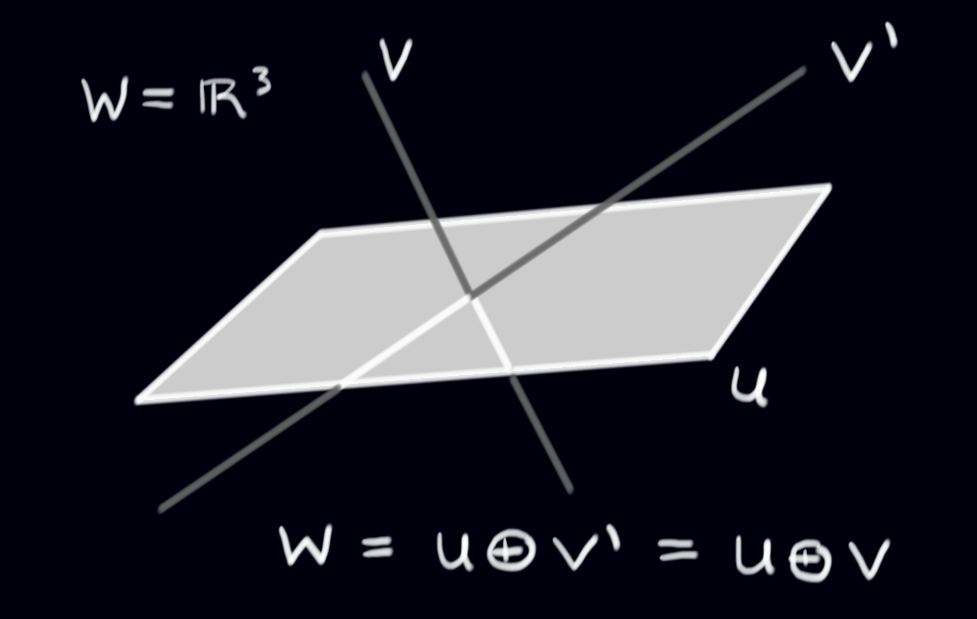
\includegraphics[scale=.25]{\gramSchmidtPath/direct_sums.jpg}
\end{center}
However, using the inner product, there is a natural candidate $U^\perp$ for this second subspace as shown here:
\begin{center}
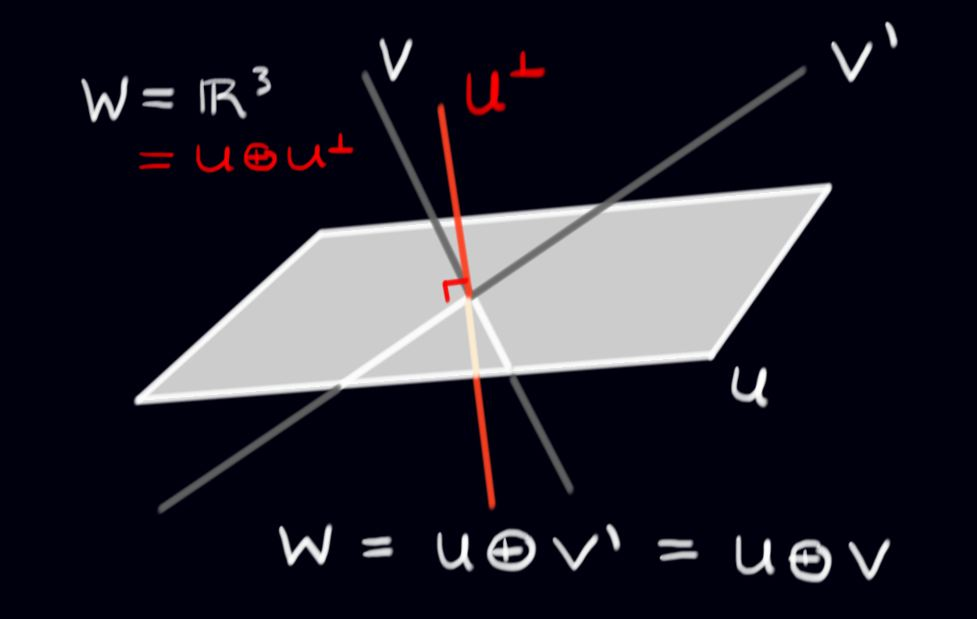
\includegraphics[scale=.25]{\gramSchmidtPath/U_perp.jpg}
\end{center}

The general definition is as follows:
\begin{definition}
Given a subspace $U$ of a vector space $W$, define:
\[
U^\perp = \{w\in W | w\dotprod u=0 \text{ for all } u\in U\}.
\]
\end{definition}

The set $U^\perp$ (pronounced ``$U$-perp'') is the set of all vectors in $W$ orthogonal to \emph{every} vector in $U$.  This is also often called the \emph{orthogonal complement}\index{Orthogonal complement} of $U$. Probably by now you may be feeling overwhelmed, it may help to watch this quick overview video:

\videoscriptlink{gram_schmidt_and_orthogonal_complements_theory.mp4}{Overview}{scripts_gram_schmidt_and_orthogonal_complements_theory}



\begin{example}
Consider any plane $P$ through the origin in $\Re^3$.  Then $P$ is a subspace, and $P^\perp$ is the line through the origin orthogonal to $P$.  For example, if $P$ is the $xy$-plane, then
\[
\Re^3=P\oplus P^\perp=\{(x,y,0)| x,y\in \Re \} \oplus \{(0,0,z)| z\in \Re \}.
\]
\end{example}

\begin{theorem}
Let $U$ be a subspace of a finite-dimensional vector space $W$.  Then the set $U^\perp$ is a subspace of $W$, and $W=U\oplus U^\perp$\index{Perp@``Perp''}.
\end{theorem}

\begin{proof}
To see that $U^\perp$ is a subspace, we only need to check closure, which requires a simple check.

We have $U\cap U^\perp=\{0\}$, since if $u\in U$ and $u\in U^\perp$, we have:
\[
u\dotprod u = 0 \Leftrightarrow u=0.
\]

Finally, we show that any vector $w\in W$ is in $U\oplus U^\perp$.  (This is where we use the assumption that $W$ is finite-dimensional.)  Let $e_1, \ldots, e_n$ be an orthonormal basis for $W$.  Set: 
\begin{eqnarray*}
u&=&(w\dotprod e_1)e_1 + \cdots + (w\dotprod e_n)e_n \in U\\
u^\perp&=& w-u
\end{eqnarray*}
It is easy to check that $u^\perp \in U^\perp$ (see the Gram-Schmidt procedure).  Then $w=u+u^\perp$, so $w\in U\oplus U^\perp$, and we are done.
\end{proof}

\reading{22}{2}
%\begin{center}\href{\webworkurl ReadingHomework22/2/}{Reading homework: problem \ref{gramschmidt}.2}\end{center}

\begin{example}
Consider any line \(L\) through the origin in \(\Re^4\). Then \(L\) is a subspace, and \(L^\perp\) is a \(3\)-dimensional subspace orthogonal to \(L\). For example, let \(L\) be the line 
$\spa \{ (1,1,1,1)^T\}$ in \(\Re^4.\) Then \(L^\perp\) is given by
\begin{eqnarray*}
L^\perp&=&\{(x,y,z,w)^T \mid x,y,z,w \in \Re \text{ and } (x,y,z,w)^T \dotprod (1,1,1,1)^T=0\} \\
&=&\{(x,y,z,w)^T \mid x,y,z,w \in \Re \text{ and } x,y,z,w=0\}.
\end{eqnarray*}
It is easy to check that 
$$
\left\{
v_1=\colvec{1\\-1\\0\\0}, v_2=\colvec{1\\0\\-1\\0}, v_3=\colvec{1\\0\\0\\-1} \right \}
$$ 
forms a basis for \(L^\perp\). We use Gram-Schmidt to find an orthogonal basis for \(L^\perp\):

First, we set \(v_1^\perp=v_1\). Then:
\begin{eqnarray*}
v_2^\perp&=&\colvec{1\\0\\-1\\0}-\frac{1}{2}\colvec{1,-1,0,0}
=\colvec{\frac{1}{2}\\ \frac{1}{2} \\-1\\ 0 },\\
v_3^\perp&=&\colvec{ 1\\0\\0\\-1} -\frac{1}{2}\colvec{1\\-1\\0\\0}-\frac{1/2}{3/2}
\colvec{ \frac{1}{2}\\\frac{1}{2}\\-1\\0} =\colvec{ \frac{1}{3}\\\frac{1}{3}\\\frac{1}{3}\\-1}.
\end{eqnarray*}
So the set \[\left\{ (1,-1,0,0)^T, \left(\frac{1}{2},\frac{1}{2},-1,0\right)^T, \left(\frac{1}{3},\frac{1}{3},\frac{1}{3},-1\right)^T \right\} \] is an orthogonal basis for \(L^\perp\).
We find an orthonormal basis for \(L^\perp\) by dividing each basis vector by its length:
\[
\left\{
\left( \frac{1}{\sqrt{2}}, -\frac{1}{\sqrt{2}},0,0 \right)^T,
\left( \frac{1}{\sqrt{6}}, \frac{1}{\sqrt{6}}, -\frac{2}{\sqrt{6}},0 \right)^T,
\left( \frac{\sqrt{3}}{6}, \frac{\sqrt{3}}{6}, \frac{\sqrt{3}}{6}, -\frac{\sqrt{3}}{2} \right)^T
\right\}.
\]
Moreover, we have
\[
\Re^4=L \oplus L^\perp = \{(c,c,c,c)^T \mid c \in \Re\} \oplus \{(x,y,z,w)^T \mid x,y,z,w \in \Re \text{ and } x+y+z+w=0\}.
\]
\end{example}

Notice that for any subspace $U$, the subspace $(U^\perp)^\perp$ is just $U$ again.  As such, $\perp$ is an involution on the set of subspaces of a vector space.

%\section*{References}
%Hefferon, Chapter Three, Section VI.2: Gram-Schmidt Orthogonalization
%\\
%Beezer, Chapter V, Section O, Subsection GSP
%\\
%Wikipedia:
%\begin{itemize}
%\item \href{http://en.wikipedia.org/wiki/Gram_schmidt}{Gram-Schmidt Process}
%\item \href{http://en.wikipedia.org/wiki/QR_decomposition}{QR Decomposition}
%\item \href{http://en.wikipedia.org/wiki/Orthonormal_basis}{Orthonormal Basis}
%\item \href{http://en.wikipedia.org/wiki/Direct_sum}{Direct Sum}
%\end{itemize}
%

\section{Review Problems}



\begin{enumerate}

\item Let $D=\begin{pmatrix}
\lambda_1 & \mc0 \\
\mc0 & \lambda_2 \\
\end{pmatrix}$.
\begin{enumerate}
\item Write $D$ in terms of the vectors $e_1$ and $e_2$, and their transposes.
\item Suppose $P=\begin{pmatrix}
a & b \\
c & d \\
\end{pmatrix}$ is invertible.  Show that $D$ is similar to
\[
M=\frac{1}{ad-bc}\begin{pmatrix}
\lambda_1ad-\lambda_2bc & -(\lambda_1-\lambda_2)ab \\[1mm]
(\lambda_1-\lambda_2)cd & -\lambda_1bc + \lambda_2ad
\end{pmatrix}.
\]
\item Suppose the vectors $\rowvec{a,b}$ and $\rowvec{c,d}$ are orthogonal.  What can you say about $M$ in this case? (Hint: think about what \(M^T\) is equal to.)
\end{enumerate}

\phantomnewpage

\item \label{orthogprob} Suppose $S=\{v_1, \ldots, v_n \}$ is an \emph{orthogonal} (not orthonormal) basis for~$\Re^n$.  Then we can write any vector $v$ as $v=\sum_ic^iv_i$ for some constants $c^i$.  Find a formula for the constants $c^i$ in terms of $v$ and the vectors in~$S$.

\Videoscriptlink{orthonormal_bases_hint.mp4}{Hint}{scripts_orthonormal_bases_hint}
\phantomnewpage

\item \label{orthogprojprob} Let $u,v$ be linearly independent vectors in $\Re^3$, and $P=\spa \{ u,v\}$ be the plane spanned by $u$ and $v$.  
\begin{enumerate}
\item Is the vector $v^\bot := v-\frac{u\cdot v}{u\cdot u}u$ in the plane $P$?
\item  What is the (cosine of the) angle between $v^\bot$ and $u$?
\item %Given your solution to the above, 
How can you find a third vector perpendicular to both $u$ and $v^\bot$?
\item  Construct an orthonormal basis for $\Re^3$ from $u$ and $v$.
\item  Test your abstract formul\ae\ starting with 
\[
u=\rowvec{1 , 2 , 0} \text{ and } v=\rowvec{0 , 1 , 1}.
\]
\end{enumerate}

\Videoscriptlink{orthonormal_bases_hint3.mp4}{Hint}{scripts_orthonormal_bases_hint3}

\phantomnewpage



\item Find an orthonormal  basis for $\Re^4$ which includes $(1,1,1,1)$ using the following procedure:\\
\begin{enumerate} 
\item Pick a vector perpendicular to the vector 
$$v_1 =\colvec{1\\1\\1\\1}$$ from the solution set of the matrix equation $$v_1^Tx=0\, .$$ Pick the vector $v_2$ obtained from the standard Gaussian elimination procedure which is the coefficient of $x_2$.
\item Pick a vector perpendicular to both $v_1$ and $v_2$ from the solutions set of the matrix equation $$\colvec{v_1^T\\[1mm]v_2^T}x=0\, .$$ Pick the vector $v_3$ obtained from the standard Gaussian elimination procedure with $x_3$ as the coefficient. 
\item Pick a vector perpendicular to $v_1,v_2,$ and $v_3$ from the solution set of the matrix equation $$\colvec{v_1^T\\[1mm]v_2^T\\[1mm]v_3^T}x=0\, .$$  Pick the vector $v_4$ obtained from the standard Gaussian elimination procedure with $x_3$ as the coefficient. 
\item Normalize the four vectors obtained   above.
\end{enumerate}


\item Use the inner product $$f\cdot g := \int_0^1 f(x)g(x)dx$$  on the vector space $V={\rm span} \{1,x,x^2,x^3\}$ to perform the Gram-Schmidt procedure on the set of vectors $\{1,x,x^2,x^3\}$. 

\item Use the inner product $$f\cdot g := \int_0^{2\pi} f(x)g(x)dx$$  on the vector space $V={\rm span} \{\sin(x),\sin(2x),\sin(3x) \}$ to perform the Gram-Schmidt procedure on the set of vectors $\{\sin(x),\sin(2x),\sin(3x) \}$. \\
Try to build an orthonormal basis for the vector space $$\spa \{ \sin(nx)~| ~n\in \N \}\, .$$
%What do you suspect about the vector space $\spa \{ \sin(nx)~| ~n\in \N \}$?\\
%What do you suspect about the vector space $\spa \{ \sin(ax)~|~ a \in \Re \}$?
\item 
\begin{enumerate}
\item
Show that if $Q$ is an orthogonal $n\times n$ matrix, then $$u\dotprod v = (Qu)\dotprod (Qv)\, ,$$ for any $u,v\in \Re^n$. That is, $Q$ preserves the inner product. 
\item Does $Q$ preserve the outer product? 
\item  If the set of vectors $\{ u_1,\dots,u_n\}$ is orthonormal and $\{ \lambda_1,\cdots,\lambda_n\}$ is a set of numbers, 
then what are the eigenvalues and eigenvectors of the matrix
$M=\sum_{i=1}^n \lambda_i u_i u_i^T$? 
\item How would the eigenvectors and eigenvalues of this matrix change if we replaced  $\{ u_1,\dots,u_n\}$ by $\{ Qu_1,\dots,Q u_n\}$?
\end{enumerate}


\item Carefully write out the Gram-Schmidt procedure for the set of vectors 
$$\left\{ \colvec{1\\1\\1}, \colvec{1\\-1\\1}, \colvec{1\\1\\-1} \right\} \, .$$ Is it possible to rescale the second vector obtained in the procedure to a vector with integer components? 


\item 
\label{basisortho}
\begin{enumerate}
\item Suppose $u$ and $v$ are linearly independent.  Show that $u$ and $v^\perp$ are also linearly independent.  Explain why $\{u, v^\perp\}$ is a basis for $\spa \{u,v\}$.



\Videoscriptlink{gram_schmidt_and_orthogonal_complements_hint.mp4}{Hint}{gram_schmidt_and_orthogonal_complements_hint}

\item Repeat the previous problem, but with three independent vectors $u,v,w$
 where $v^\perp$ and $w^\perp$ are as defined by the Gram-Schmidt procedure. 
\end{enumerate}

\phantomnewpage


\item \label{QRprob} Find the $QR$ factorization of
$$
M=\begin{pmatrix}1&0&\phantom{\!-}2\\-1&2&0\\-1&-2&2
\end{pmatrix}\, .
$$

\phantomnewpage

\item Given any three vectors $u,v,w$, when do $v^\perp$ or $w^\perp$ of the Gram--Schmidt procedure vanish?

\phantomnewpage

\item For $U$ a subspace of $W$, use the subspace theorem to check that $U^\perp$ is a subspace of $W$.

\phantomnewpage


\phantomnewpage

\item %(Extra Credit) 
Let $S_n$ and $A_n$ define the space of $n \times n$ symmetric and anti-symmetric matrices, respectively. These are subspaces of the vector space $M^n_n$ of all $n\times n$ matrices. What is $\dim M^n_n$, $\dim S_n$, and $\dim A_n$? Show that $M^n_n = S_n + A_n$. Define an inner product on square matrices
$$
M\cdot N ={\rm tr} MN\, .
$$
Is $A_n^{\perp}=S_n$? Is $M^n_n = S_n \oplus A_n$?

%\emph{Hint: Note that $\dim S_n = \dim U_n$ where $U_n$ is the vector space of all $n \times n$ upper triangular matrices, and also note that $\dim A_n = \dim \widetilde{U}_n$ where $\widetilde{U}_n$ is the vector space of all strictly $n \times n$ upper triangular matrices (\emph{i.e.} the diagonal entries are all 0).}

\item The vector space $V={\rm span} \{ \sin(t),\sin(2t), \sin(3t) , \sin(3t)\}$ has an inner product: 
$$f\cdot g:=\int _0^{2\pi}f(t)g(t) dt\, .$$ Find the orthogonal compliment to $U={\rm span} \{ \sin(t)+\sin(2t) \}$ in $V$. Express $\sin(t)-\sin(2t)$ as  the sum of vectors from $U$ and $U^\perp$.

\end{enumerate}

\phantomnewpage

\newpage

